% Insert in Experimental setup. Compile from the repository root.
\begin{figure*}[t]
\centering
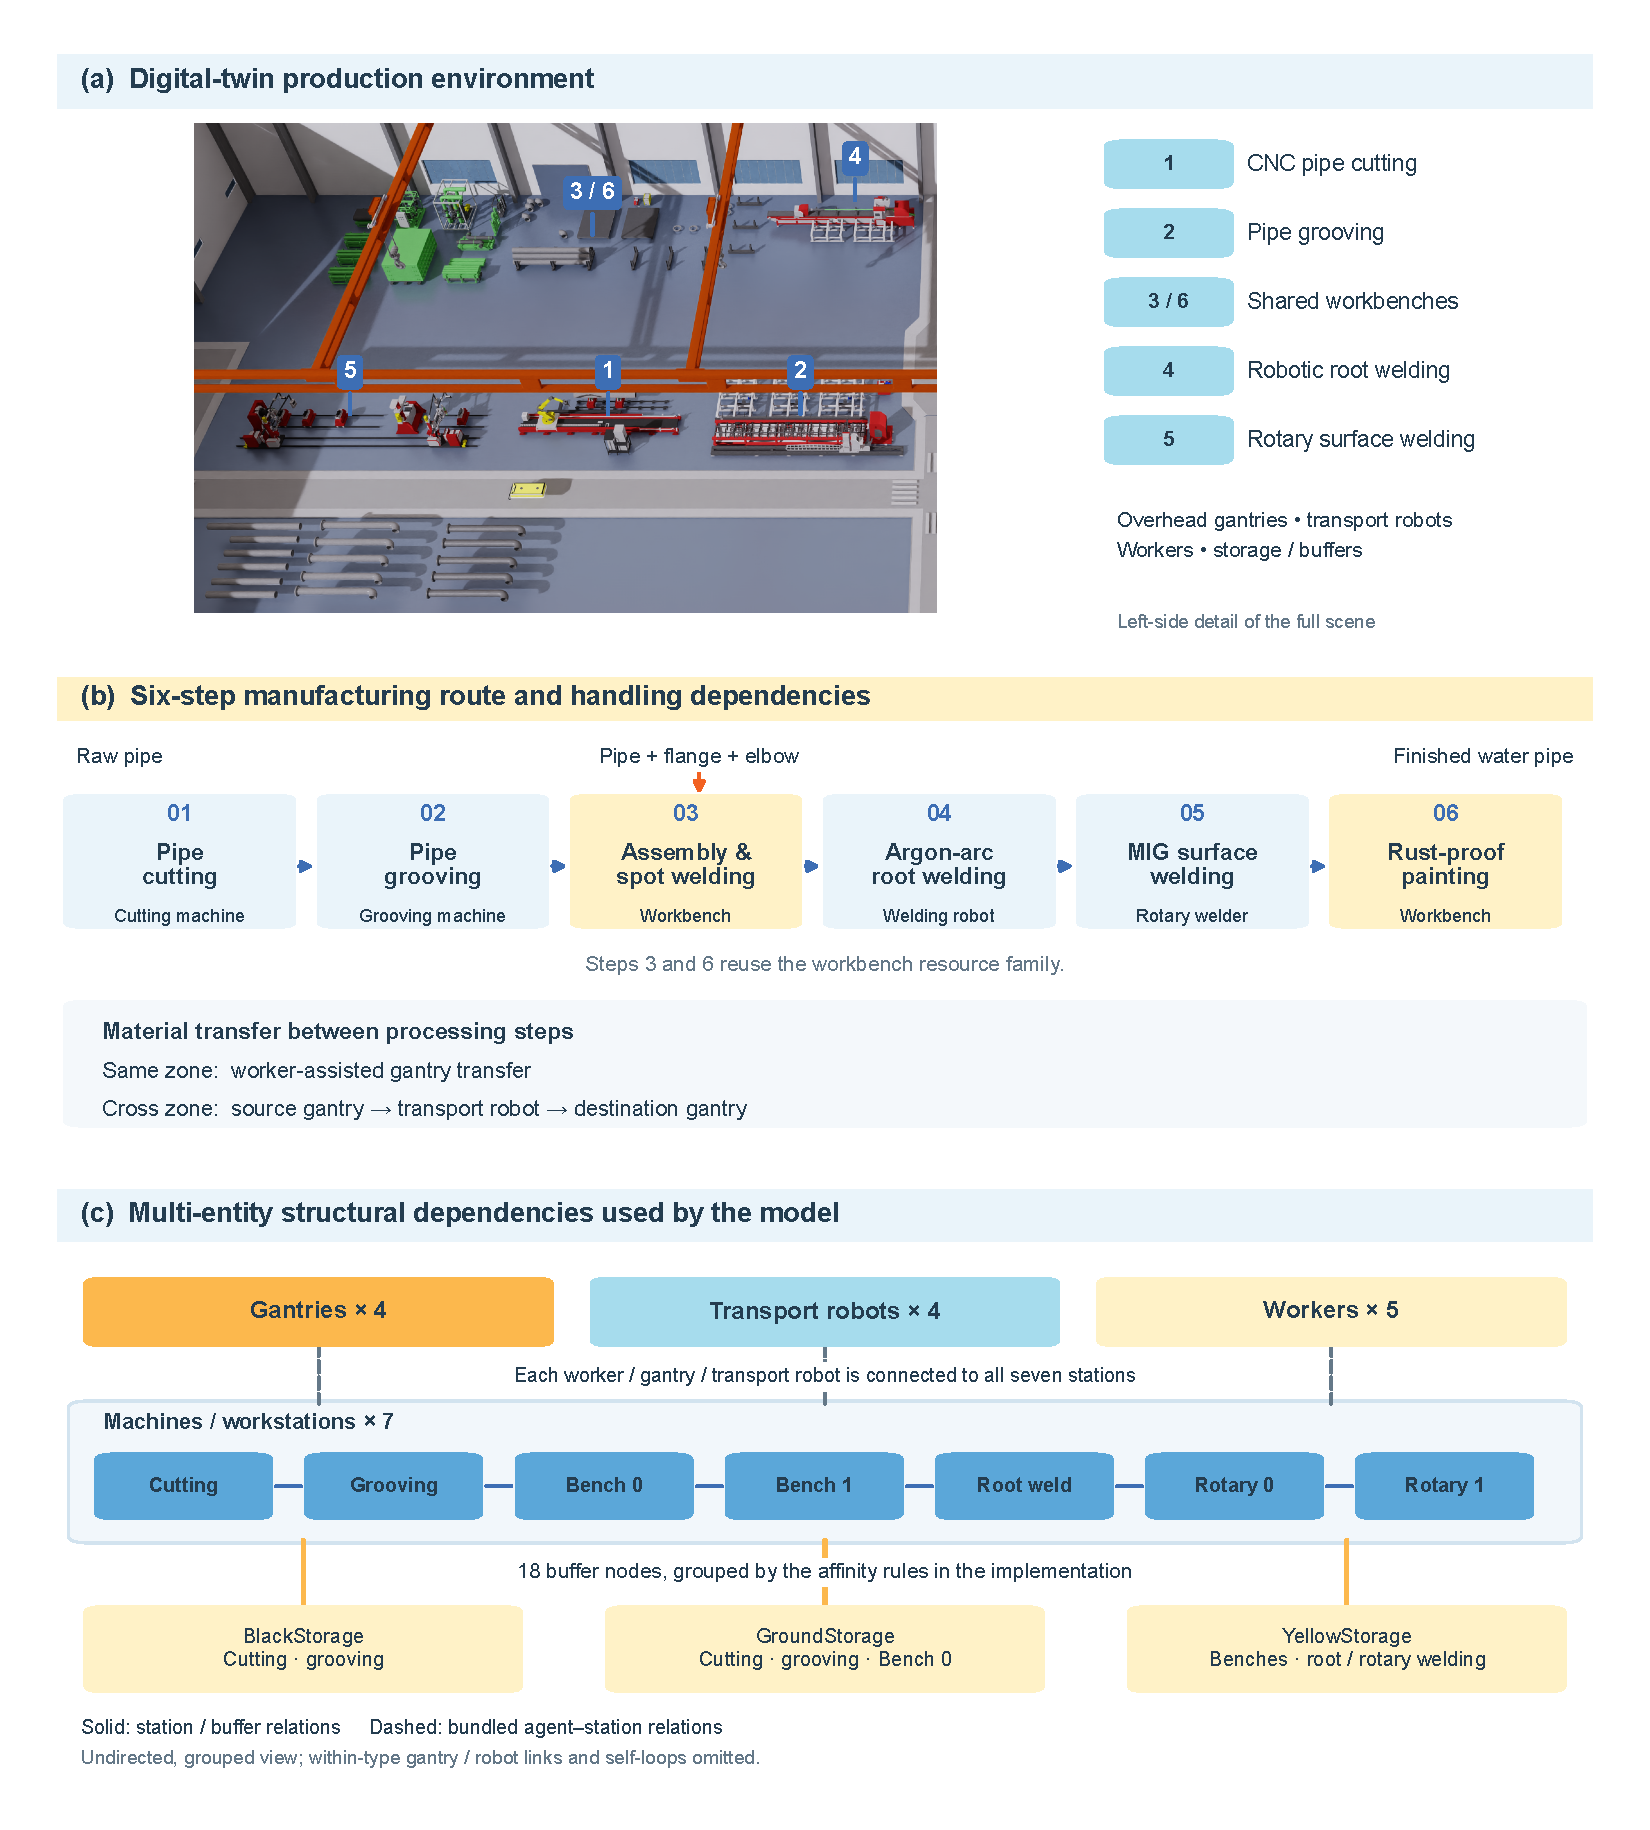
\includegraphics[width=0.96\textwidth]{figures/fig_factory_process_entities.pdf}
\caption{Digital-twin production environment, manufacturing route, and multi-entity dependencies. (a) Detail of the left-hand production area; equipment numbers refer to the six processing steps in (b). Steps 3 and 6 share the workbench resource family. Handling within a zone uses a gantry, while cross-zone transfer uses source and destination gantries with a transport robot. (c) Grouped view of the implemented undirected factory graph, comprising seven workstations, four gantries, four transport robots, five workers, and eighteen buffers. Agent--station connections are bundled; buffer labels specify their station affinities. Within-type gantry and robot links and self-loops are omitted for clarity. The workstation graph is a structural prior, not the directed manufacturing route.}
\label{fig:factory-process-entities}
\end{figure*}
